\documentclass{llncs}
\usepackage{graphicx}
\usepackage{url}
%\usepackage[utf8]{inputenc} % Umlaute (währinger straße)
\usepackage[T1]{fontenc}

\begin{document}

<<<<<<< HEAD
%\title{Evaluation of a Visualization Component for the Difference Graph}
\title{A User Evaluation of Different Visual Representations for Visualizing Differences in Process Models}

=======
\title{Evaluation of a Visualization Component for the Difference Graph}
>>>>>>> origin/master
\author{Firstname Lastname \and Firstname Lastname}
\institute{Universit\"at Wien \\ W\"ahringer Strasse 29 \\ 1090 Wien}
\maketitle

\begin{abstract}
<<<<<<< HEAD
Finding differences between two processes can be a complex, time consuming, and expensive task. Our work is based on the difference graph approach which calculates the differences between two process models. In this paper we evaluate different possibilities for visualizing these differences. For this purpose we have selected some common visual elements such as color, font size, and line stippling and evaluated these different representations with 31 participants through an online survey. Our results show that color coding was the preferred method of the participants for depicting difference in a graph visualization.
\end{abstract}

\begin{keywords}
	Difference Graph, Visualization, Processes, Process Model
=======
Finding differences between two processes can be a complex, time consuming and expensive task. Our work is based on the difference graph which calculates the differences of two process models. We want to extend the model with and expressive visualization to show where differences can be found. In order to find the best suiting visualization we extracted several visualizations from literature. These visualization were the foundation of an evaluation. The result showed that color coding suits the difference graph visualization best.
\end{abstract}

\begin{keywords}
	Difference Graph, Visualization
>>>>>>> origin/master
\end{keywords}


%Todo:
% Update Images -> Resolution, Font and Visuals
% Read everything

\section{Introduction}
\label{sec:Introduction} % [1 Page]

<<<<<<< HEAD
Processes are an indispensable part of today's businesses. From visualizing processes for communication, up to optimization companies constantly use processes to gain additional business intelligence.

%What is the problem / how is it solve by now
Using process mining algorithms on data collected during process execution allows for further analysis~\cite{lit:PMDiscoveryConformanceEnhancement} such as detection of bottlenecks, problems, and violations. Conformance checking~\cite{lit:ConformanceCheckingOfProcesses} is a part of process mining which assesses if a log file deviates from a process model. Unfortunately conformance checking focuses only on detection of deviations between log files and process models. Kriglstein et al.~\cite{lit:VisuApprDiffAnalysis}, on the other hand, computed the difference model between two process variants and visualized the resulting differences using [XXX] notation. The input models iteself can be generated through process mining or created manually. Visualizing data is a very important task to enhance the users understanding of the data. However, Kriglstein et al.~\cite{lit:VisuApprDiffAnalysis} did not evaluate how to best visualize the differences to allow for an effective interpretation.

%Contribution
In this work we address this issue by investigating which visual depictions of differences suit the interpretation of differences in process models best. To answer this question we conducted an online survey with company employees and students and nine different representations gathered through a literature search.

%Applications
Difference calculation and visualization can be used for different applications in business process management. For example, to compare process models generated with process mining techniques from two processes. This helps finding deviations between these processes. Consider, for example, a company which executes the same task at two different locations. Unfortunately in one location the execution takes twice as long. Comparing the process models of these locations can reveal why the execution time is doubled. When comparing two process models one can also gain additional information if these processes can be merged. Finding deviations allows to determine where problems may occur. Another area of application is to assess one process at different points in time. For example, to evaluate how one process has evolved from one year to the next. 

%Section overview
The remainder of this paper is structured as follows. Section 2 gives an overview of the difference graph model and its calculation as well as an outline why visualization is beneficial. Section 3 covers our evaluation. Related work is shortly discussed in Section 4. Section 5 concludes this paper including possible directions for future work.


%\textit{Literature to solve this problem}
%Current process mining methods are able to check for compliance (check rule violation while or after the process is executed) and conformance (compare a log with a process model).
%In some cases it is not useful to compare real world process logs with handcrafted process models. What if two real world processes should be compared?
%This question answer \cite{lit:VisuApprDiffAnalysis} with the introduction of their difference graph model. They presented the model and essential parts for calculation. However they do not evaluate how to visualize this model. Visualizing data is a very important task to enhance the users understanding of the data.
=======
Processes are an indispensable part of today’s business. From visualizing processes for communication, up to optimization we constantly use processes to gain additional business intelligence.

%What is the problem / how is it solve by now
Using process mining algorithms on data collected during process execution allows further analysis \cite{lit:PMDiscoveryConformanceEnhancement}, for example, detection of bottlenecks, problems and violations. Conformance checking \cite{lit:ConformanceCheckingOfProcesses} is a part of process mining which allows to check if a log file deviates from a process model. Unfortunately conformance checking focuses only on detection of deviations between log files and process models. With their paper \cite{lit:VisuApprDiffAnalysis} introduced the difference graph which allows to check for differences between two process models. These models can be generated through process mining or even crafted by hand. 
However they do not evaluate how to visualize the difference model. Visualizing data is a very important task to enhance the users understanding of the data. 

%Contribution
In this work we investigate the following research question: Which visualization suites the difference graph best? To answer this we conduct a literature research to find different representations. Afterwards we use a survey to evaluate which of the found visualizations should be used for representing the difference graph.

%Applications
Difference calculation and visualization can be used in different areas of application. One is to compare process models generated with process mining techniques from two processes. This helps finding deviations between those processes. For example, a company with two locations executes the same task. Unfortunately in one location the execution takes twice the time. Comparing the process models of these locations can help finding why the execution time is doubled. When comparing two process models one can although gain additional information if those processes can be merged. Finding deviation allows to determine where problems may occur. Another area of application is to use one process at different points in time. For example, compare the years 2013 and 2014 of one process. This allows to see how the process has evolved.

%Section overview
In Section 2 we give an overview of the difference graph model and calculation. As well as an outline why the visualization is important. To select an appropriate visualization Section 3 covers our evaluation process. Related work can be found in Section 4. Section 5 concludes this paper with a reference where future work can be done.


>>>>>>> origin/master

%\textit{Literature to solve this problem}
%Current process mining methods are able to check for compliance (check rule violation while or after the process is executed) and conformance (compare a log with a process model).
%In some cases it is not useful to compare real world process logs with handcrafted process models. What if two real world processes should be compared?
%This question answer \cite{lit:VisuApprDiffAnalysis} with the introduction of their difference graph model. They presented the model and essential parts for calculation. However they do not evaluate how to visualize this model. Visualizing data is a very important task to enhance the users understanding of the data.

<<<<<<< HEAD
\section{Difference Graph Model and Visualization} % [2 Pages]
\label{sec:DiffgraphModel}
The difference graph concept~\cite{lit:VisuApprDiffAnalysis} consists of two parts: the model and the visualization of the model. In this section we will first describe the difference model and then focus on visualizing this model.

Elementary component for the difference graph model is a process model. Following~\cite{lit:VisuApprDiffAnalysis} a process model can be viewed as a directed connected graph $PM = (N, E \subseteq N \times N)$ where $N$ is a set of nodes and $E$ is a set of directed control edges. Each node has a unique identifier, a label, and a type (e.g., activity, event, or gateway node). Optionally, nodes and edges may have weights assigned which represent the instance traffic. Instance traffic measures how often a specific activity is executed in real world. A process model consists of one start node which has no incoming edges and one end node which has no outgoing edges. Except from start and end node each node is connected by at least one incoming and outgoing edge. Every node has to be on a path between start and end node. As an example, Figure~\ref{fig:ProcessModels} shows two versions of a process model. When visually comparing these two variants one can observe that, for example, that $B$ has been deleted from the right model while a new node $E$ has been added. However, with increasing size of the model, manually finding the differences and commonalities can become increasingly cumbersome and time-consuming.
=======

\section{Difference Graph Model and Visualization} % [2 Pages]
\label{sec:DiffgraphModel}
The difference graph concept \cite{lit:VisuApprDiffAnalysis} consists of two parts one is the model and the other is the visualization of this model. In this section we will  first describe the difference model and then take a journey towards visualizing this model.

Elementary component for the difference graph model is a process model. According to \cite{lit:VisuApprDiffAnalysis} a process model is defined as a direct connected graph \textit{PM} = (\textit{N}, \textit{E} $\subseteq$ \textit{N} $\times$ \textit{N}). \textit{PM} consist of nodes \textit{N} and direct control edges \textit{E}. Each node consists of an unique identifier, label and a type.
The process model consists of one start node which has no incoming edges and one end node which has no outgoing edges. Except from start and end node each node is connected by at least one incoming and outgoing edge. Every node has to be on a path between start and end node. Figure \ref{fig:ProcessModels} shows two process models. Input1 consists of four weighted edges and four labeled nodes. Input2 consists of three edges and although four labeled nodes. Interesting examples for difference calculation of these two inputs are node C where the weight has increase from 2 to 3, node B and E which are only visible in one of the inputs.
>>>>>>> origin/master

\begin{figure}
	\centering
	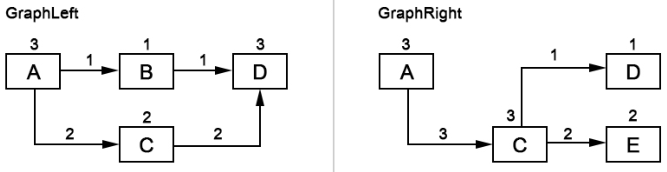
\includegraphics[width=0.8\textwidth]{Images/ProcessModels.PNG}
	\caption{Two process models.}
	\label{fig:ProcessModels}
\end{figure}

For generating the difference graph two process models are needed. These models can be described in many different process modeling languages, for example, Petri Nets~\cite{lit:Petrinet}, UML~\cite{lit:UML}, EPC~\cite{lit:EPC}. Generally, all languages which allow to view a process as (weighted) directed graph can be used for the difference graph calculation. For this purpose, the method takes two graphs as input, in the following referred to as $PM_1$ and $PM_2$, and generates a new graph $PM_2 - PM_1$ with markings associated with its nodes and edges (for an in-depth discussion see~\cite{lit:VisuApprDiffAnalysis}). The following list shows the different markings and describes in which case these markings are assigned.

<<<<<<< HEAD
\begin{description}
	\item[\textsc{New}] a node/edge is marked as \textsc{New} if the node/edge was added from $PM_1$ to $PM_2$.
	\item[\textsc{Positively changed}] a node/edge is marked as \textsc{Positively changed} when the weight has increased from $PM_1$ to $PM_2$.
	\item[\textsc{Unchanged}] a node/edge is \textsc{Unchanged} if it appears in both input models (and has the same weights).
	\item[\textsc{Negatively changed}] a node/edge is marked as \textsc{Negatively changed} when the weight has decreased in $PM_2$.
	\item[\textsc{Deleted}] a node/edge is mark as \textsc{Deleted} if the node/edge was deleted from $PM_2$.
\end{description}
=======
For generating the difference graph two process models are needed. These models can be described in many different process modeling languages e.g. Petri Nets \cite{lit:Petrinet}, UML \cite{lit:UML}, EPC \cite{lit:EPC}. All of those languages which are conform to the above mentioned process model description can be used for the difference graph calculation. From both input process models the difference graph model is calculated. This model extends a process model with an element called marking. The marking is applied on edges and nodes and is generated during the calculation process.
>>>>>>> origin/master

As a side note it should me emphasized that the markings are only used if the input models have weights assigned to nodes and edges.

<<<<<<< HEAD
Figure~\ref{fig:DiffGraphCalculation} shows the resulting graph when the left model in Figure~\ref{fig:ProcessModels} is subtracted from the right model. For example, Node $B$ was deleted from $PM_2$ and therefore is marked as \textsc{deleted} while the weight of node $C$ has increased from 2 to 3 and thus $C$ has been marked as \textsc{Positively changed}. 
=======
For calculating the markings the first model is subtracted from the second one. During the calculation three or five different markings can be generated. Five markings can be calculated if the input process models consist of weights. If not, only three markings can be calculated. The following list shows all five markings and gives a description in which case they are used. 

\begin{itemize}
	\item \textbf{New}, a node/edge gains the marking New when the node/edge was added from Input1 to Input2.
	\item \textbf{Positively changed}, a node/edge is marked as Positively changed when the weight has increased from Input1 to Input2.
	\item \textbf{Unchanged}, a node/edge gains this marking when its value matches in both inputs.
	\item \textbf{Negatively changed}, a node/edge is marked as Negatively changed when the weight has decreased from Input1 to Input2.
	\item \textbf{Deleted}, a node/edge gains the marking Deleted when the node/edge was deleted from Input1 to Input2.
\end{itemize}

Hint the markings positively changed and negatively changed can not be calculated if the input process models do not consist of weights.

Figure \ref{fig:DiffGraphCalculation} shows the results for subtracting Input2 from Input1 which were shown in Figure \ref{fig:ProcessModels}. Node B  was deleted from Input2 therefore, the marking deleted is applied the weight is calculated by subtracting 1 from 0 = -1. Node C was changed positively the weight has increased from 2 to 3.
>>>>>>> origin/master

\begin{figure}
	\centering
	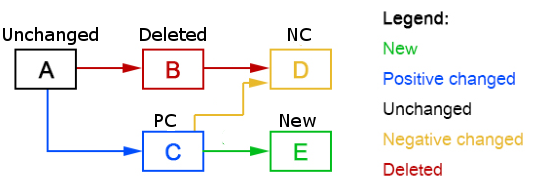
\includegraphics[width=0.8\textwidth]{Images/ResultGraph.PNG}
<<<<<<< HEAD
	\caption{Calculating the differences from Figure~\ref{fig:ProcessModels} leads to this difference graph. On top of each edge and node calculated weights and applied markings are shown.}
	\label{fig:DiffGraphCalculation}
\end{figure}

The main focus of this paper is how to best visualize the difference graph to promote an effective interpretation by users. The basic idea is to depict the various markings differently, for example, by using icons or color-coding. To do so we conducted an evaluation which is shown in the next section.

=======
	\caption{Calculating the differences from Figure \ref{fig:ProcessModels} leads to this difference graph. On top of each edge and node calculated weights and applied markings are shown.
	%TODO: change all colors to Black and state on top of each node and edge which marking is applied. This will lead to the following: first the reader sees the two inputs, then he/she sees the calculation and later on in the evaluation he/she sees how this markings which are stated here with text are visualized.
	}
	\label{fig:DiffGraphCalculation}
\end{figure}

The main  focus of this paper is how to visualize the difference graph. The idea behind the visualization of the difference graph is to represent each of the markings with different styles. For example, each marking can be mapped to represent a specific symbol. This symbol can then be visualized on nodes and edges.

A survey was conducted to secure a good understanding of the difference graph visualization. To do so a literature research with the goal to find different visualization approaches was executed. Our first step was to find relevant keywords addressing the topic of difference visualization. These keywords where used within search engines. This led to a wealth of papers which where used as a basis for snowballing method where on one side other relevant papers where collected and on the other side new keywords where extracted. From all collected papers we were able to extract nine visualization approaches. These nine approaches were used in our evaluation.

This section gave an overview about the fundamental process model which is the base for the difference graph model. We showed how the difference graph model is calculated and which markings can be expressed on edges and nodes. For visualizing the model an appropriate style for markings has to be found which will be part of the next section.
>>>>>>> origin/master

\section{Evaluation} %  [5 Pages]
\label{sec:Evaluation} % [1/2 Page]
To address the research question, stated in Section 1, an online survey was conducted. We used the information found with literature research as input for our survey. The survey should show which from the found visualizations fits the difference graph best.

\subsection{Literature Research} % [1/2 Page]
\label{sec:LitResearch}
In order to identify different visual possibilities to distinguish between different markings we conducted a literature search. Our first step was to find relevant keywords addressing the topic of difference visualization. These keywords where used within the search engines Google scholar and Microsoft academic. This led to nine paper which where used as a basis for snowballing method where on one side other relevant paper where collected and on the other side new keywords where extracted, all used keywords are shown in table \ref{table:Keywords}. Overall snowballing led to additional 22 paper. We read those 31 paper and extracted every visualization which allows five different styles. Five styles are necessary to be able to visualize each marking with an own style e.g. different colors, shapes, symbols. From all collected papers we were able to extract nine visualization approaches. Figure \ref{fig:visualizations} shows all nine approaches used in our evaluation.

\begin{table}
	\centering
		\begin{tabular}{|p{4cm}|p{4cm}|p{4cm}|}
			\hline
			Graph differences & Calculate graphical differences & Matrix difference calculation 	\\
			\hline
			Delta Analysis & Union of Models &  Difference computation 	\\
			\hline
			Visual Difference computation & UML diagram differences &  Merging business processes 	\\
			\hline
			Merging processes  & Structural differences between graphs & Visual graph comparison 	\\
			\hline
			Visualizing Differences between Graphs & Change detection & Change visualization 	\\
			\hline
			Graph evolution visualization & Visualization properties &  	\\
			\hline
		\end{tabular}
		\vspace{10pt}
\caption{List of keywords used for literature research.}
\label{table:Keywords}
\end{table}

\begin{figure}
	\centering
	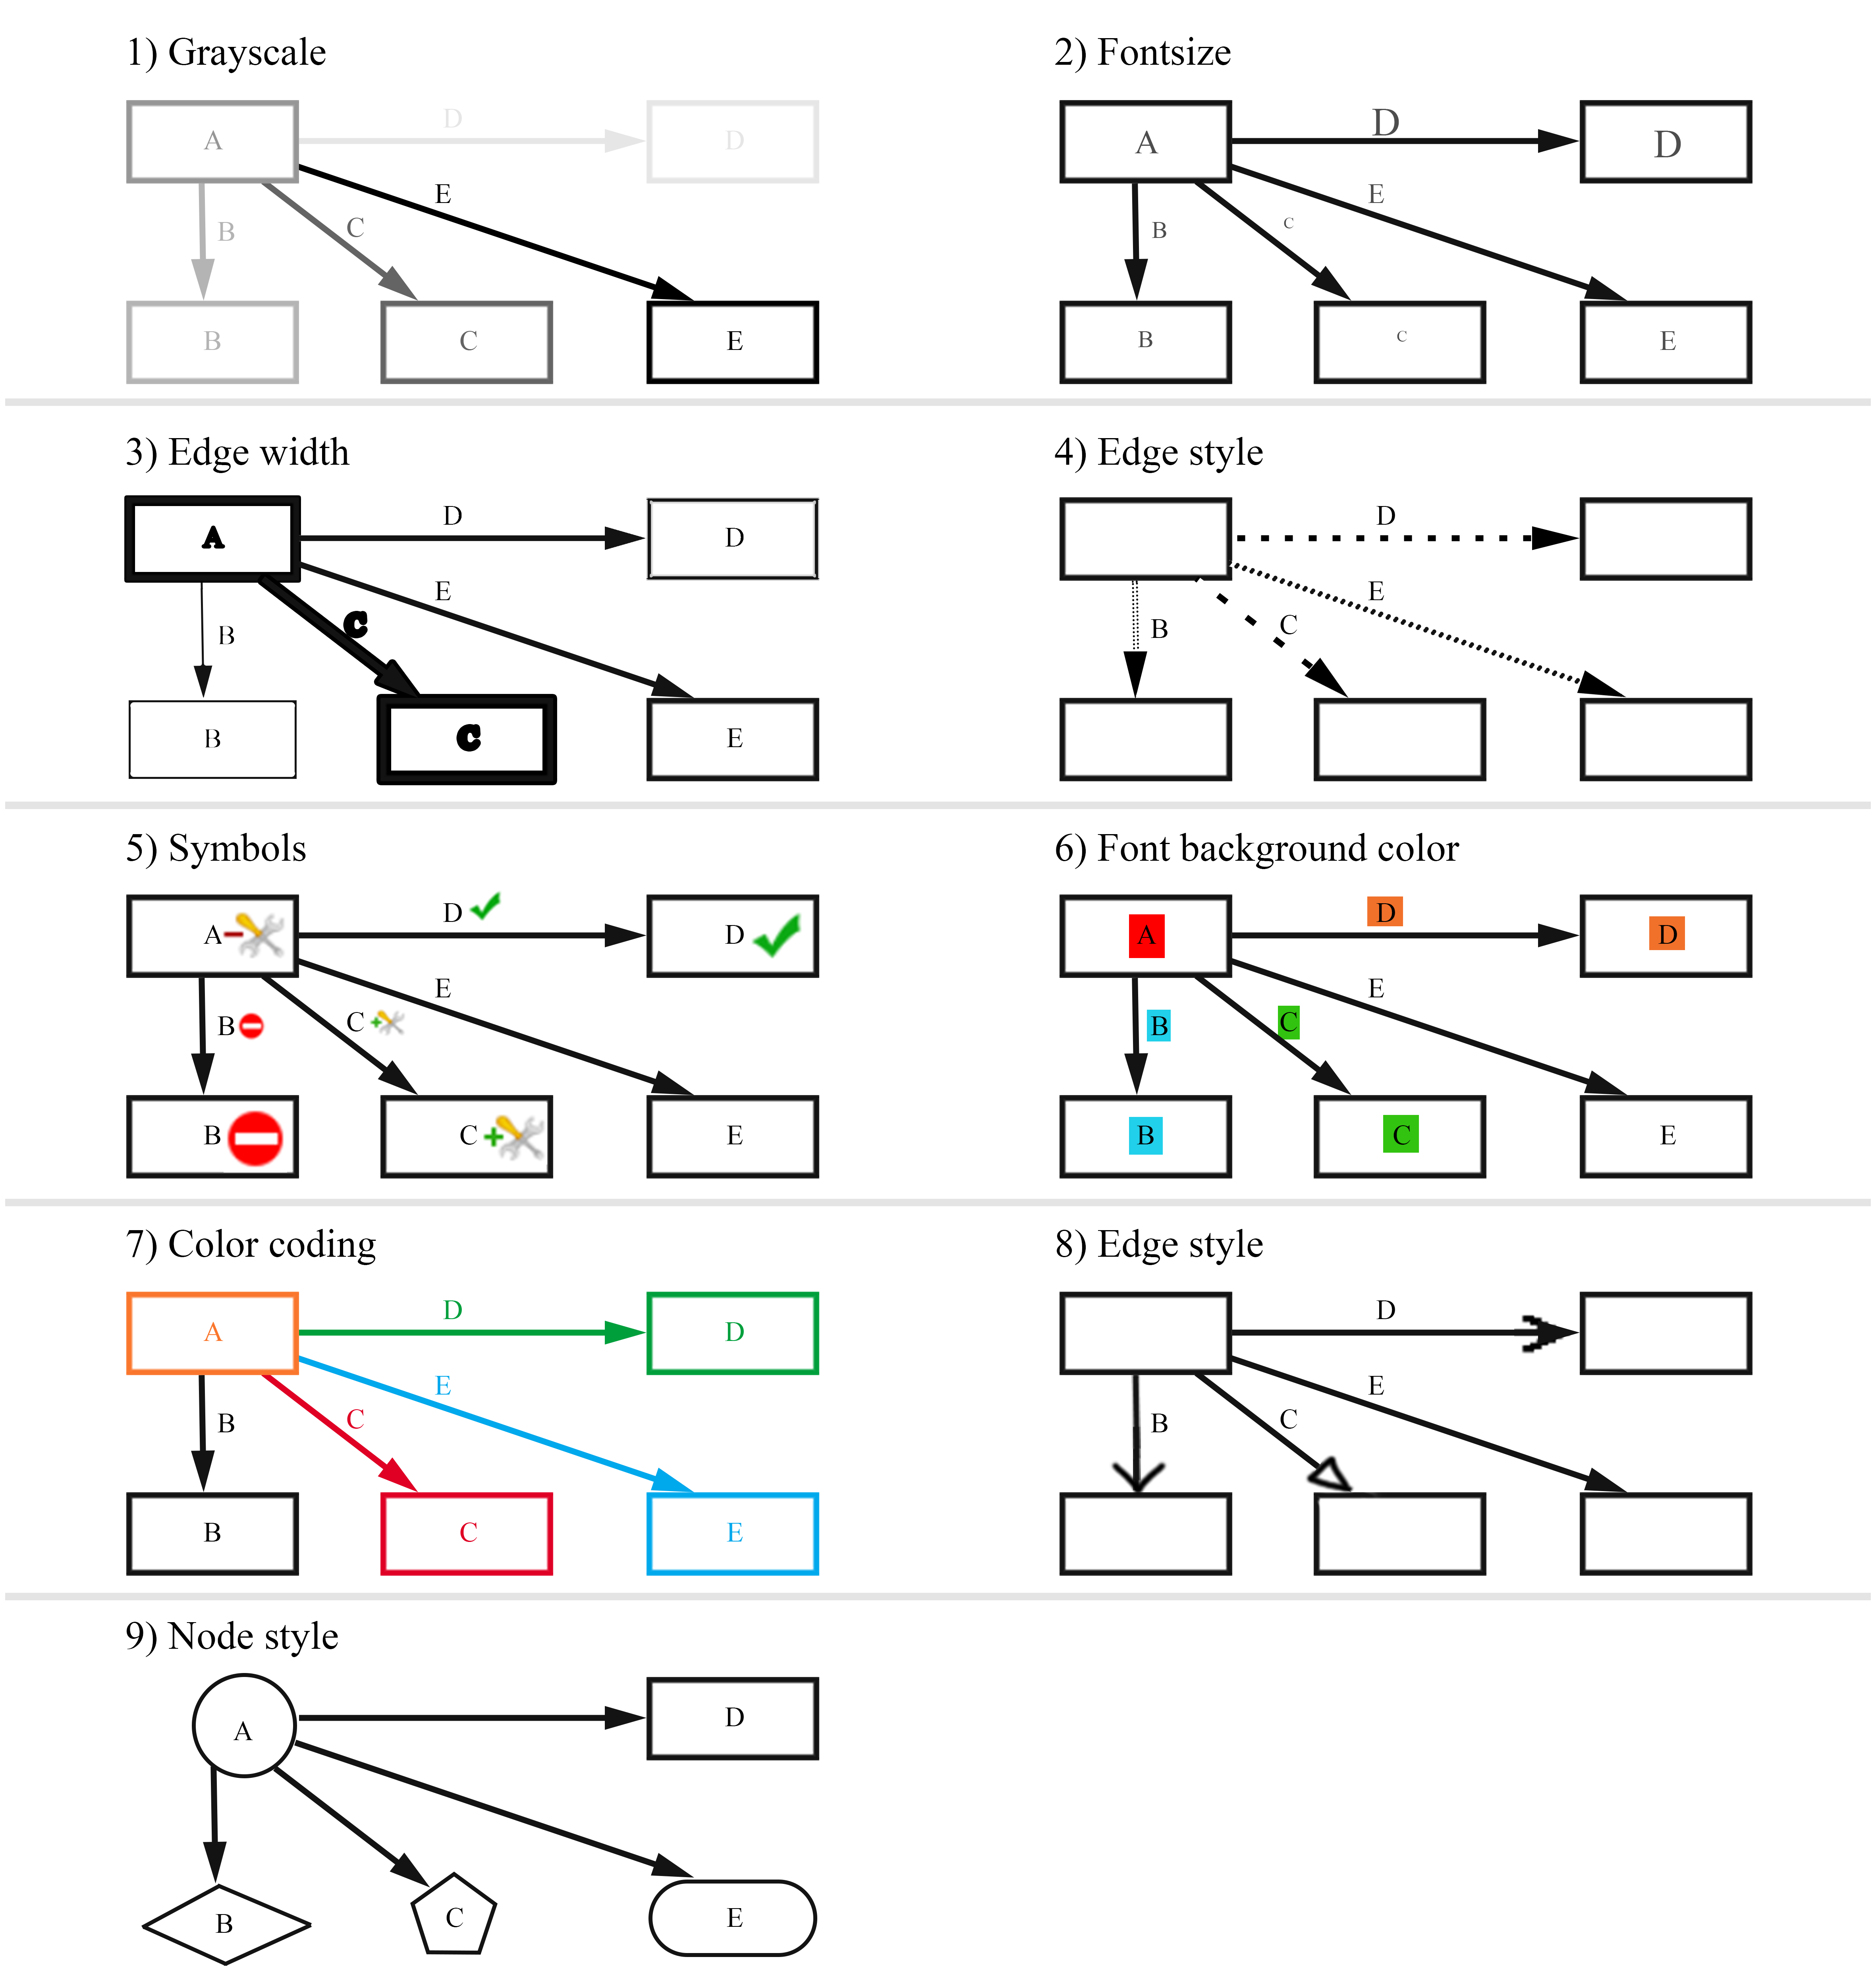
\includegraphics[width=350px]{Images/Overview.PNG}
	\caption{Visualizations}
	\label{fig:visualizations}
\end{figure}


\subsection{Design} % [1/2 Page]
\label{sec:Design}
<<<<<<< HEAD
To avoid massive scrolling and simplify navigation through the survey we used single pages. Single pages come with the advantage that on each commit of a page we are able to validate the answers and give hints to the user where answers are missing. Overall the survey was divided into three groups: introduction, styles, and advanced/demographic questions.
=======
To avoid massive scrolling and simplify navigation through the survey we used single pages. Single pages come with the advantage that on each commit of a page we are able to validate the answers and give hints to the user where answers are missing. Overall the survey is divided into three groups introduction, styles and advanced/demographic questions.

The introduction gives an example how the difference graph is calculated and asks the user a question specific to this example. This question allows to check if the user understood the example or not. Further questions on the introduction page check the attendees knowledge about graphs.
>>>>>>> origin/master

The introduction gave an example how the difference graph is calculated and contained a question specific to this example to verify if the participant has understood the difference graph concept or not. Further questions on the introduction page asked about knowledge about graphs.  

Following the introduction are questions about the visualizations themselves. Each visualization represents each of the five markings in a different way. For example, the visualization \emph{Color coding} uses the colors green, blue, black, orange, and red to distinguish between the markings. Each of this visualizations is presented on a single page which contains two questions related to the visualization. One question required the participants to rate the expressiveness of the visualization on a scale from [TODO]. The second question asked the participants to assign each visual element to the marking for which they think the element is best suited. For example, the participants had to assign a red colored node to the marking they deem most suitable for it, such as \textsc{Deleted}.

In the advanced/demographic section we asked the participants to rank the visualizations according to their expressiveness. In addition, participants were asked if they prefer to use the same visual representation regardless of the graph's size or if the representation should be determined by the size of the graph. On our last page participants where asked if they have worked with business processes before. Afterwards the survey concluded with demographic questions about, for example, age, gender, and employment. 

\subsection{Procedure} % [1/2 Page]
\label{sec:Procedure}

<<<<<<< HEAD
First, a two-stage pretest to validate the design of the survey was conducted to ensure the questionnaire is understandable and time required to complete the survey is adequate. In the first pretest a discussion with two people took place to asses the wording of the questionnaire. After changing the survey the user feedback a second pretest with five participants was conducted. During their survey they where encouraged to think aloud, to ask questions, and to provide feedback for possible improvements. All their questions and comments where noted and analyzed after the pretest. After finishing the second pretest minor changes to the questions were made. 
=======
In the first pretest a discussion with two people took place where the overall question and answer wording was adapted to support the users understanding.

In our second pretest five attendees had to complete the survey and give advices what should be changed. During their survey they where encouraged to think aloud and ask questions. All their questions and comments where noted and analyzed after the pretest. After finishing the second pretests minor changes to answers where made. This changes should secure a better understanding and reduce the surveys duration.

After finishing the pretests the URL to the survey was distributed by E-Mail to 159 people working in companies and studying in universities. Additionally the URL was posted on Facebook addressing students. Overall 103 attendees opened the survey from whom 31 attendees finished.
>>>>>>> origin/master

After finishing the two pretests the link to the survey was distributed by e-mail to 159 company employees and students. Additionally the link was posted on Facebook addressing students on an private group initiated from and for business informatics students with 537 likes. Overall 73 attendees started the survey from whom 31 attendees finished. Incomplete surveys were excluded from our analysis. In the end, we received 31 complete responses.

\subsection{Results and Discussion} % [2-3 Pages]
\label{sec:Results}

Our participants where spread  from 19 to 46 years. One participant was below 20 years, 11 participants where in range from 20 to 25 years, although 11 participants from 26-30, one was 36 years, three where 44 and one 46 years. Three people did not fill in their age. We had 24 men (77.4 \%), 6 women (19.4 \%) and 1 participant with no answer, participating in the survey. Overall 19 participants (61.3 \%) had worked with graphs before and 12 participants (38.7) had not. As expected a little less participants had worked with process models. From 31 participants 13 (41.9 \%) had worked with process models, 17 (54.8 \%) had not worked with process models before and one participant (3.2 \%) did not answer the question.

Before we go into details which representation should be used for the difference graph we want to show that the difference graph can be understood by novices as well as experienced persons. 61.3\% of the participants understood the concept by the very first example. Another analysis shows that 73.6\% of the participants with fundamental graph knowledge understood the example. In contrast, only 41.6\% of the participants without graph knowledge understood the example.

To find the best suiting representation we analyze the intuitive understanding and the ranking for each style. The intuitive understanding is important to allow users to gain an overview of the visualization without the need to look which marking is represented by which style. The goal is to find a visualization where each style can be intuitively allocated to a marking.

%Table with Mean value and Deviation 
\begin{table}
\centering
\begin{tabular}{|l|l|l|l|}
	\hline
	Visualization & Mean value  & Max value  & Min value \\
	\hline
	Name & 2 & 3 & 4 \\
	\hline  
\end{tabular}
\caption{Intuitive understanding}
\label{tab:IntuitiveUnderstanding}
\end{table}

Table~\ref{tab:IntuitiveUnderstanding} shows a list of all visualizations in terms of intuitive understanding. On top of the list is the visualization \emph{Symbols} followed by \emph{Color coding} and \emph{Background color}. The maximum intuitive understanding possible is 31, which can only be achieved if every participant assigns the same style to the marking. Symbols range from 27 to 29 with a mean value of 27,6. For example, the green tick (Figure \ref{fig:visualizations}.5 Symbols)  was assigned by 27 participants as marking \textsc{New}. Color coding has a mean value of 25,4 and \emph{Background color} of 23,6.

\begin{figure}
	\centering
	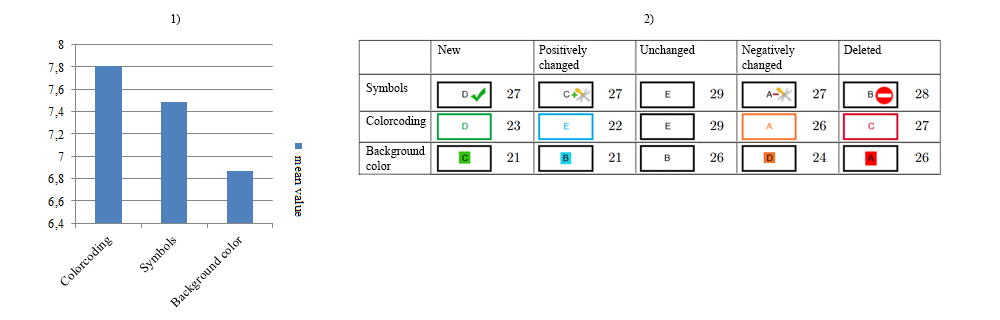
\includegraphics[width=350px]{Images/Results.PNG}
	\caption{Ranking of all styles with standard deviation.}
	\label{fig:SurveyResults}
\end{figure}



After seeing all visualization approaches the users task was to order them according to their expressiveness. The ranking was transformed into numbers best ranking counts 9 worst 1. To compare the rankings the mean-value is calculated. Figure~\ref{fig:SurveyResults} shows the mean value for all representations. As before the figure shows the representations \emph{Color coding}, \emph{Symbols} and \emph{Background color}. This time the order is different now \emph{Color coding} is on top followed by \emph{Symbols} and \emph{Background color}.


Within both evaluations only three of nine visualizations are on top. \emph{Background color} was found in both evaluations on third place. Participants commented that \emph{Background color} is alike \emph{Color coding} with the hint that \emph{Color coding} is more useful then \emph{Background color}. Participants mentioned \emph{Color coding} is more pleasant to look at and more suitable for small as well as big graphs. While \emph{Background color} is not suitable for big graphs. The reason for this is \emph{Background color} only colorizes the label of a node. In big graphs finding the correct label for a node can be challenging. Therefore only the visualizations \emph{Color coding} and \emph{Symbols} are considered for further analysis.

Both visualizations offer advantages over the other. For \emph{Symbols} the same negative aspect as for \emph{Background color} can be encountered. Within big graphs finding the symbol assigned to a specific edge can be challenging. One solution would be to change visualizations with the size of the graph. Our evaluation showed that only 29\% of the participants recommend to change the visualization with the graphs size.

We consider \emph{Color coding} as the best visualization. The visualization offers a good intuitive understanding, scored best in the overall ranking and is suitable for small and big graphs. As commented by our participants we recommend using a legend to show which color represents which marking.

Figure~\ref{fig:DiffGraphVisualization} shows an example how the final representation can look. The figure shows the graph which was calculated in the previous example with applied color coding.

\begin{figure}
	\centering
	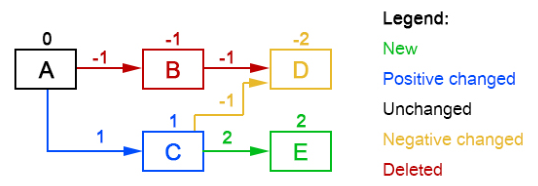
\includegraphics[width=0.8\textwidth]{Images/ColorCodedGraph.PNG}
	\caption{Color coded representation of the difference graph}
	\label{fig:DiffGraphVisualization}
\end{figure}

\section{Related Work}  % [1/2 Page]
\label{sec:RelatedWork}

<<<<<<< HEAD
Conformance checking~\cite{lit:ConformanceCheckingOfProcesses} is a part of process mining~\cite{lit:PMDiscoveryConformanceEnhancement,lit:BusinnessProcessMiningAnIndustrialAppliction} which deals with detection of inconsistencies between a process model and a log file. Conformance checking lacks of the possibility to compare two process models generated from log files. Kriglstein et al.~\cite{lit:VisuApprDiffAnalysis} proposed the difference graph concept where instance traffic of two processes is compared. They implemented a prototype where differences are visualized through color coding. They did not evaluate if color coding is a suitable option for visualizing differences within process models.

One of the first visualization approaches for process models where Petri Nets~\cite{lit:Petrinet}. Since then many different languages emerged~\cite{lit:UML,lit:EPC,lit:YAWL}. From process mining perspective the topic of visualization has also been addressed in~\cite{lit:ProMFramework}. For the difference graph we need to show one process model which visualizes the differences of two process models. Therefore we extend previous work in this field by evaluating how differences can be visualized within process models.
=======
Conformance checking \cite{lit:ConformanceCheckingOfProcesses} is a part of process mining \cite{lit:BusinnessProcessMiningAnIndustrialAppliction,lit:PMDiscoveryConformanceEnhancement} which deals with detection of inconsistencies between a process model and a log file. Conformance checking lacks of the possibility to compare two process models generated from log files. \cite{lit:VisuApprDiffAnalysis} proposed the difference graph concept where instance traffic of two processes is compared. They implemented a prototype where differences are visualized through color coding. They did not evaluate if color coding is a suitable option for visualizing differences within process models.

One of the first visualization approaches for process models where Petri Nets \cite{lit:Petrinet}. Since then many different languages emerged \cite{lit:YAWL,lit:UML,lit:EPC}. From process mining perspective the topic of visualization has also been addressed in \cite{lit:ProMFramework}. For the difference graph we need to show one process model which visualizes the differences of two process models. Therefore we extend previous work in this field by evaluating how differences can be visualized within process models.
>>>>>>> origin/master

\section{Conclusion} %  [1/2 Page]
\label{sec:Conclusion}
In our work we combine the difference graph concept with a visualization component. In the concept paper for the difference graph, color coding was mentioned as the preferred method for visualization. In our survey color coding was one of nine styles which can be used for difference visualization. Our evaluation confirmed there thoughts and showed that color coding is the best method for visualizing differences between two process models. To support the users intuitive understanding we suggest to use a legend which states the meaning of each color.

<<<<<<< HEAD
With these results in hand a prototype implementation of the difference graph concept enhanced with color coding was implemented within the ProM framework. The plug in is currently available in the nightly build of ProM.

The color coded visualization is not limited to only show differences between two process models. Color coding can be applied to show differences in many scenarios. For example, conformance and compliance checking which both in some way try to find differences.

=======
The color coded visualization is not limited to only show differences between two process models. Color coding can be applied to show differences in many scenarios. For example, conformance and compliance checking which both in some way try to find differences.

>>>>>>> origin/master
Future work in terms of visualization can be done in several areas. Process models often allow clustering but how does clustering affect the color coded visualization? Our approach only visualizes differences between two models. Therefore another interesting topic would be the visualization of process evolution. 

\bibliography{Literature}
\bibliographystyle{plain}

\end{document}
